\documentclass{../../../../style/mkimain}

\series{4}
\month{květen}
\year{2023}

\begin{document}
\ExecuteMetaData[../../problems/problem4-K/problem4-K.tex]{header}
\noindent\ExecuteMetaData[../../problems/problem4-K/problem4-K.tex]{task}
\proborigin{}
\klein
De Broglieho teorie dualismu se využívá v elektronových mikroskopech, které se skládají z elektronového paprsku a
elektromagnetických čoček a fungují analogicky ke světelným mikroskopům.
Obecně je zvětšení mikroskopu závislé na vlnové délce použitého \uv{měřiče}, a proto, že elektrony s velmi vysokou
energií mohou mít až $100\,000$ krát menší vlnovou délku než světlo, můžeme pod elektronovým mikroskopem vidět objekty o 
několik řádů menšího měřítka, například i jednotlivé atomy.

\begin{figure}[H]
    \begin{center}
    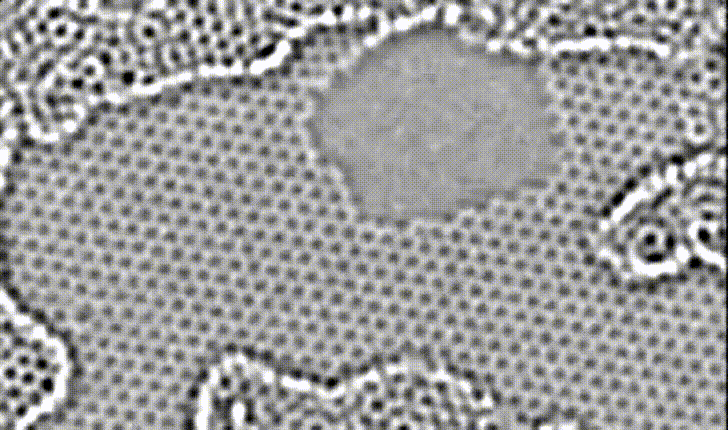
\includegraphics[scale=0.37]{grafen.png}\\
    \vspace{0.15cm}
        Obr. 1: Jednotlivé atomy uhlíku v jednoatomové vrstvě grafenu
    \end{center}
\end{figure}
\end{document}
